\documentclass[12pt]{article}


% Math		****************************************************************************************
\usepackage{fancyhdr} 
\usepackage{amsfonts}
\usepackage{amsmath}
\usepackage{amsthm}
\usepackage{dsfont}

% Macros	****************************************************************************************
\usepackage{calc}

% Commands	****************************************************************************************
%\newcommand{\problem}[1]{\hspace{-\widthof{#1}} \textbf{#1}}
\newcommand{\problem}[1]{\hspace{-4 ex} \large \textbf{#1}\\}
\newcommand{\reverseconcat}[3]{#3#2#1}

%page		****************************************************************************************
\usepackage[margin=1in]{geometry}
\usepackage{setspace}
\doublespacing
\pagestyle{fancy}
\fancyhf{}
\rhead{Shaw \space \thepage}
\setlength\parindent{0pt}

%Code		****************************************************************************************
\usepackage{listings}
\usepackage{courier}
\lstset{
	language=Python,
	showstringspaces=false,
	formfeed=newpage,
	tabsize=4,
	commentstyle=\itshape,
	basicstyle=\ttfamily,
}

%Images		****************************************************************************************
\usepackage{graphicx}
\graphicspath{ {images/} }


\begin{document}
	\thispagestyle{empty}
	
	\begin{flushright}
		Sage Shaw \\
		m565 - Fall 2017 \\
		\today
	\end{flushright}
	
{\large \textbf{HW 2}}\bigbreak

\problem{1 (a)}\\
	Code for secant method in python follows:
	\singlespacing
	\begin{lstlisting}
def secant(f, x0, x1, epsilon=1e-16, n_max=10**5):
	xs = [x0,x1]
	xn = x1
	xn_1 = x0
	fn = f(xn)
	fn_1 = f(xn_1)
	for i in range(n_max):
		if abs(fn) < epsilon:
			return xs
		xn, xn_1 = xn - (xn-xn_1)/(fn-fn_1)*fn, xn
		fn, fn_1 = f(xn), f(xn_1)
		xs.append(xn)
	return None
	\end{lstlisting}
	\doublespacing
	
\problem{1 (b)}\\
	Code for Newton's method in python follows:
	\singlespacing
	\begin{lstlisting}
def newton(f, df, x0, epsilon=1e-16, n_max=10**5):
	x = x0
	xs =[x]
	fx = f(x)
	dfx = df(x)
	for i in range(n_max):
		if abs(fx) < epsilon:
			return xs
		x = x - fx/dfx
		xs.append(x)
		fx, dfx = f(x), df(x)
	return None
	\end{lstlisting}
	\doublespacing
\problem{1 (c)}\\
	The output for the secant method is below.
	\begin{center}
		\begin{tabular}{|c|c|c|c|}
			\hline
			$n$&$x_n$&relative error&rate\\ \hline
			1&5.5&8.6977255889355&N/A\\ \hline
			2&5.25&8.256919880347523&N/A\\ \hline
			3&0.0294863000416&0.948009082466&-0.0252912792622\\ \hline
			4&0.823978157018&0.452857101461&14.8372523985\\ \hline
			5&0.593254095941&0.0460391685359&3.88581886785\\ \hline
			6&0.565982615568&0.00204652838394&2.01139762445\\ \hline
			7&0.567148753391&9.63245318171e-06&1.86548763383\\ \hline
			8&0.567143291557&2.02338959262e-09&1.73314683194\\ \hline
			9&0.56714329041&4.89392647061e-15&1.64601718863\\ \hline
		\end{tabular}
	\end{center}
	It's somewhat difficult to tell with so few iterations, but the rate of convergence appears to be approaching the golden ratio as expected.

	The output for Newton's method is below.
	\begin{center}
	    \begin{tabular}{|c|c|c|c|}
	    	\hline
	    	$n$&$x_n$&relative error&rate\\ \hline
	    	1&5.25&8.256919880347523&N/A\\ \hline
	    	2&0.0326257855847&0.942473469868&-0.0280654002561\\ \hline
	    	3&0.507891082956&0.104474845169&38.1249608767\\ \hline
	    	4&0.566496637787&0.00114019267083&3.00005806752\\ \hline
	    	5&0.56714321473&1.33440892109e-07&2.33593620286\\ \hline
	    	6&0.56714329041&5.08968352943e-15&2.07911417502\\ \hline
	    \end{tabular}
	\end{center}
    It's somewhat difficult to tell with so few iterations, but it appears to be converging quadratically as expected.
    
\problem{2 (a)}
	Assume that $f$ has a root at $x^*$. Define $\epsilon_n = x^*-x_n$ for each $x_n$. Then $0 = f(x^*) = f(x_n + \epsilon_n)$. By Taylor series expanding around $x_n$ we get that 
	$$
	0 = f(x_n + \epsilon_n) \approx f(x_n) + \epsilon_n f^\prime(x_n) + \frac{\epsilon_n^2}{2}f^{\prime\prime}(x_n)
	$$
	or equivalently
	\begin{align}\label{p2a1}
	\epsilon_n \approx -\frac{f(x_n)}{f^\prime(x_n)} - \frac{\epsilon_n^2f^{\prime\prime}(x_n)}{2f^\prime(x_n)}
	\end{align}
	If we then assume that $\epsilon_n^2 \approx 0$, we can say that $\epsilon_n \approx \frac{-f(x_n)}{f^\prime(x_n)}$. Substituting into the right side of (\ref{p2a1}) we get 
	$$
	x^* - x_n = \epsilon_n \approx -\frac{f(x_n)}{f^\prime(x_n)} - \frac{f(x_n)^2f^{\prime\prime}(x_n)}{2f^\prime(x_n)^3}
	$$
	which gives us the recurrance relation
	$$
	x_{n+1} = x_n -\frac{f(x_n)}{f^\prime(x_n)} - \frac{f(x_n)^2f^{\prime\prime}(x_n)}{2f^\prime(x_n)^3}
	$$
	
\problem{2 (b)}
	\textbf{use computer lab}
	
\problem{3 (a)}
	If $r=1-\frac{x^2}{a}$ then $\sqrt{a} = x(1-r)^{-\frac{1}{2}}$. \\
	Then the iteration $x_{n+1} = x_n(1-r)^{-\frac{1}{2}}$ where $r=1-\frac{x_n^2}{a}$ will converge in one step. If we Taylor expand $f(r) = (1-r)^{-\frac{1}{2}}$ around $r=0$ we get
	$$
	f(r) = (1-r)^{-\frac{1}{2}} \approx 1 + \frac{1}{2}r
	$$
	Substituting back $r=1-\frac{x_n^2}{a}$ we get $f(1-\frac{x_n^2}{a}) \approx 1 + \frac{1}{2} (1-\frac{x_n^2}{a}) = \frac{1}{2}(3-\frac{x_n^2}{a})$. Then our iteration becomes $x_{n+1} = \frac{x_n}{2}(3-\frac{x_n^2}{a})$. This is essentially using newton's method to calculate the root of $f(r) = (1-r)^{-\frac{1}{2}}$ which will converge quadratically and thus we can expect this recurance to converge quadratically as well. My Python implementation follows.
	\singlespacing
	\begin{lstlisting}
def my_sqrt(a, x0, epsilon=1e-15, n_max=10**5):
	xs = [x0]
	x = x0
	for i in range(n_max):
		if abs(x**2 - a) < epsilon:
			return xs
		x = x/2 * (3 - x**2/a)
		xs.append(x)
	return  None
	\end{lstlisting}\doublespacing
	
	The output can be seen below for $a=2$ and $x_0=1$. After a few iterations the number of accurate digits almost doubles at each iteration, consistent with quadratic convergence.
	
	\begin{center}
		\begin{tabular}{|c|c|c|c|}
			\hline
			$n$&$x_n$&abs err&ratio\\ \hline
			1&1&0.414213562373&N/A\\ \hline
			2&1.25&0.164213562373&2.04974089911\\ \hline
			3&1.38671875&0.0274948123731&1.98925208746\\ \hline
			4&1.413416936993599&0.000796625379496&1.98542199024\\ \hline
			5&1.4142128893918142&6.72981280925e-07&1.99177257226\\ \hline
			6&1.4142135623726146&4.80504525058e-13&1.99583740676\\ \hline
			7&1.4142135623730951&0.0&N/A\\ \hline
		\end{tabular}
	\end{center}
	
\problem{3 (b)}
	In Figure 1 can be seen equation (3) from the homework: $y=\frac{1}{2}(x+\frac{a}{x})$.
	\begin{figure}[h]
		\caption{$y=\frac{1}{2}(x+\frac{a}{x})$ and $y=x$}
		\centering
		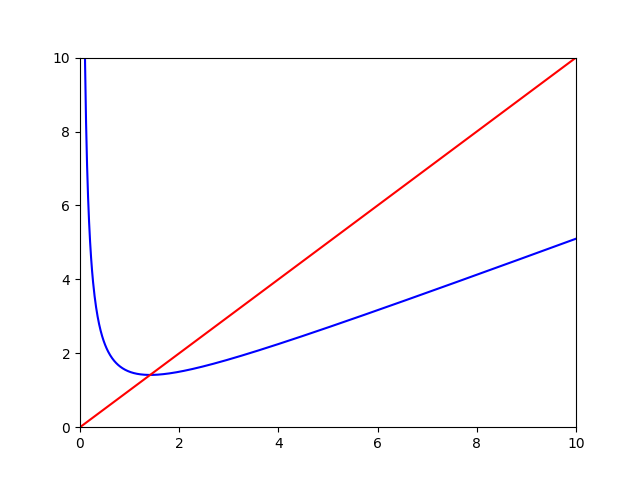
\includegraphics[width=0.5\textwidth]{hw2_figure_1}
	\end{figure}\\
	Note, that for a square-root, only a positive valued initial guess is appropriate. From the graph, one would expect that all choices of starting point will converge. The table below confirms this suspicion. 
	\begin{center}
		\begin{tabular}{|c|c|}
			\hline
			$x_0$&converged\\ \hline
			0.0001&1.414213562373095\\ \hline
			1&1.414213562373095\\ \hline
			2&1.414213562373095\\ \hline
			4&1.414213562373095\\ \hline
			100&1.414213562373095\\ \hline
		\end{tabular}
	\end{center}
	
	In Figure 2 can be seen equation (4): $y=\frac{x}{2}(3-\frac{x^2}{a})$.
	\begin{figure}[h]
		\caption{$y=\frac{x}{2}(3-\frac{x^2}{a})$ and $y=x$}
		\centering
		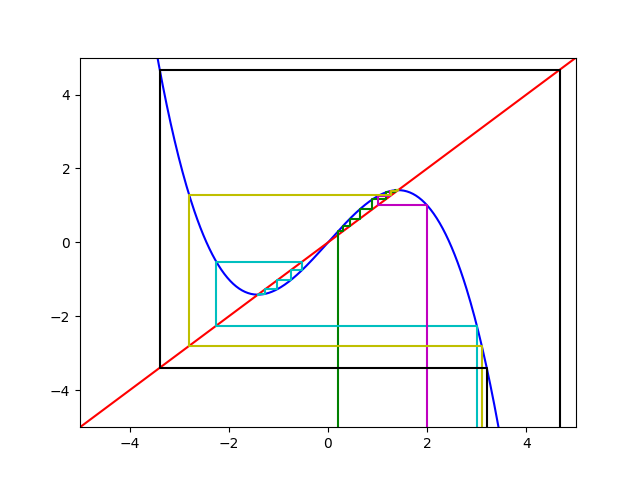
\includegraphics[width=0.5\textwidth]{hw2_figure_2}
	\end{figure}
	
	\begin{center}
		\begin{tabular}{|c|c|}
			\hline
			$x_0$&converged\\ \hline
			-100&249850.0\\ \hline
			-10&-3244116.25\\ \hline
			-5&9094925797.771563\\ \hline
			-1.82674185835&-1.41421356237\\ \hline
			-1.82474185835&-1.41421356237\\ \hline
			-1&-1.414213562373095\\ \hline
			-0.01&-1.4142135623730951\\ \hline
			0.01&1.4142135623730951\\ \hline
			1&1.414213562373095\\ \hline
			1.82474185835&1.41421356237\\ \hline
			1.82674185835&1.41421356237\\ \hline
			2&1.414213562373095\\ \hline
			5&-9094925797.771563\\ \hline
			10&3244116.25\\ \hline
			100&-249850.0\\ \hline
		\end{tabular}
	\end{center}
	
\problem{3 (c)}
	Notice that similarly to above, $\frac{1}{\sqrt{a}}=x(1-r)^{-\frac{1}{2}}$ where $r=1-ax^2$ is an identity for any positive value of $x$. We then Taylor expand the function $f(r)=(1-r)^{-\frac{1}{2}}$ about $r=0$ to get the following
	$$
	f(r) \approx 1 + \frac{1}{2}r + \frac{3}{8}r^2
	$$
	Substituting $r=1-ax^2$ we get
	\begin{align*}
		f(1-ax^2) & \approx 1 + \frac{1}{2}(1-ax^2) + \frac{3}{8}(1-ax^2)^2\\
		& \approx 1 + \frac{1}{2} - \frac{a}{2}x^2 + \frac{3}{8}(1-2ax^2 + a^2x^4) \\
		& \approx 1 + \frac{1}{2} - \frac{a}{2}x^2 + \frac{3}{8} -\frac{6}{8}ax^2 + \frac{3}{8}a^2x^4) \\
		& \approx \frac{15}{8} - \frac{10}{8}ax^2 + \frac{3}{8}a^2x^4\\
		& \approx \frac{1}{8}(15 - 10ax^2 + 3a^2x^4)\\
		& \approx \frac{1}{8}(15 - ax^2(10 - 3ax^2))
	\end{align*}
	Then our iteration becomes
	\begin{align*}
		x_{n+1} & = x_nf(1-ax_n^2) \\
		x_{n+1} & = \frac{x_n}{8}(15 - ax_n^2(10 - 3ax_n^2))
	\end{align*}
	as desired. \textbf{explain why cubicly convergent} \\
	
	\singlespacing
	\begin{center}
		\begin{tabular}{|c|c|}
			\hline
			$x0$&converges to\\ \hline
			-3.2&diverges\\ \hline
			-3.1&-1.41421356237\\ \hline
			-3.0&1.41421356237\\ \hline
			-2.9&1.41421356237\\ \hline
			-2.5&1.41421356237\\ \hline
			-2.4&-1.41421356237\\ \hline
			-0.1&-1.41421356237\\ \hline
			0.1&1.41421356237\\ \hline
			2.4&1.41421356237\\ \hline
			2.5&-1.41421356237\\ \hline
			3.0&-1.41421356237\\ \hline
			3.1&1.41421356237\\ \hline
			3.2&diverges\\ \hline
			3.3&diverges\\ \hline
		\end{tabular}
	\end{center}
	\doublespacing
	

\problem{5 (a)}
	From the table below it can be seen that that the iteration occilates between 0.9948 and 0.0117. Obviously niether of these are a solution to our problem since the next iteration returns the other number for each.
	\singlespacing
	\begin{center}
		\begin{tabular}{|c|c|}
			\hline
			$n$&$x_n$\\ \hline
			1&0\\ \hline
			2&0.9953222650189527\\ \hline
			3&0.010556209425946548\\ \hline
			4&0.9948670503002457\\ \hline
			\vdots & \vdots \\ \hline
			26&0.9948153975507391\\ \hline
			27&0.011699975456613668\\ \hline
			28&0.9948153975507384\\ \hline
			29&0.011699975456615172\\ \hline
			30&0.9948153975507384\\ \hline
		\end{tabular}
	\end{center}
	\doublespacing
	
\problem{5 (b)}
	Python implementation of Steffenson's iterative method:
	\singlespacing
	\begin{lstlisting}
def foo_6(x):
	return -1*erf(2*(x-1))
	
def hw2_p5b():
	xs = [0]
	x = 0
	ns = [0]
	#perform first iteration so that 
#error checking can compute
	g = foo_6(x)
	x = x - (g-x)**2/(foo_6(g) -2*g + x)
	xs.append(x)
	for i in range(1,1000000): 
		if abs(xs[-1] - xs[-2]) < 1e-15:
			break
		g = foo_6(x)
		if abs((foo_6(g) -2*g + x)) < 1e-15:
			break
		x = x - (g-x)**2/(foo_6(g) -2*g + x)
		xs.append(x)
		ns.append(i)
	latex_table((ns, xs),('$n$', '$x_n$'))
	\end{lstlisting}
	\doublespacing
	Iterations of Steffenson's iterative method are in the the table below.
	\begin{center}
		\begin{tabular}{|c|c|}
			\hline
			$n$&$x_n$\\ \hline
			0&0\\ \hline
			1&0.5003142541320008\\ \hline
			2&0.6395901752177244\\ \hline
			3&0.661032522348998\\ \hline
			4&0.6615598346647998\\ \hline
			5&0.6615601506706955\\ \hline
			6&0.661560150670809\\ \hline
		\end{tabular}
	\end{center}

\problem{5 (c)}
	From the fundamental theorem of calculus 
	$$
	\frac{d}{dx}\text{erf}(x) = \frac{d}{dx}\frac{2}{\sqrt{\pi}}\int_0^x e^{-t^2}dt = \frac{2}{\sqrt{\pi}} e^{-x^2}
	$$
	Using this and applying the chain rule, we arive at the derivative of $g(x) = -\text{erf}(2(x-1))$ \\
	$$
	g^\prime(x) = -\frac{4}{\sqrt{\pi}} e^{-x^2}
	$$
	Evaluating at our fixed point $x^* = 0.661560150670809$ we obtain $g(x^*) = -1.4272696617560152$. Since the magnitude of this derivative is not less than 1, we are not guaranteed convergence by the Fixed Point theorem.
	
	
\problem{6} 
	Suppose we have a function $f(x)$, such that for any $x_0$, an iteration of Newton's method returns $-x_0$. That is 
	$$
	-x_0 = x_0 - \frac{f(x)}{f^\prime(x)}
	$$
	It then follows that $2x_0 = \frac{f(x)}{f^\prime(x)}$. Letting $f(x)=y$, we can then manipulate it as follows
	\begin{align*}
		\frac{1}{y}\frac{dy}{dx} & = \frac{1}{2x} \\
		\int \frac{1}{y}\frac{dy}{dx} dx & = \int \frac{1}{2x} dx \\
		\int \frac{1}{y}dy & = \frac{1}{2}\int \frac{1}{x} dx \\
		ln\vert y \vert & = \frac{1}{2} ln\vert x \vert + C_0 \\
		ln\vert y \vert & = ln\vert x \vert^\frac{1}{2} + C_0 \\
		\vert y \vert & = C_1 \vert x \vert^\frac{1}{2} \\
		y & = \pm C_1 \sqrt{\vert x \vert} \\
	\end{align*}
	Noticing that the derivative is undefined at $x=0$ we allow for separate solutions when $x$ is either positive or negative. When checking it is quickly shown that $f(x)=C_1 \text{sign}(x)\sqrt{\vert x \vert}$.


\end{document}
